% !TeX root = ../main.tex
% Add the above to each chapter to make compiling the PDF easier in some editors.
\chapter{Related Work}\label{chapter:related-work}

\subsection{Classification of location data and apps that use it}
In order to review existing approaches and research, classify location aware services by the acceptable delay of the location information being available:
\begin{itemize}
  \item Almost no delation tolerance: e.g. an application showing a pop-up about a nearby venue e.g. a coffe shop when a pedestrian passes
  \item Some delay e.g. one minute is acceptable: An application e.g. google maps derives the information of congested traffic from devices reporting their GPS data which show lower than usual speed. As congestions worth reporting last longer than one minute, some delay in the device's information reaching the server is acceptable.
  \item Significant delay of hours, days or even weeks is acceptable for historical and statistical use of location data e.g. to find out about popular visiting times
\end{itemize}

\subsection{What has been achieved so far}

Most existing approaches focus on publishing location data where a huge delay is acceptable as can be seen in the following table: TODO [create table].

\section{Inferring data from already published datasets}
\begin{itemize}
	\item privacy issues
	\begin{itemize}
		\item Centralized databases also expose the users to a security risk (through theft) \parencite{iot, hoh2006enhancing}.
		\item Research has shown, that even from a location data set that is pseudonymous, i.e. the identifiers have been stripped or anonymized from the data, it is still possible to infer the home location of single users through inference attacks \parencite{krumm, cellphone, privacy-home-work-pairs, hoh2006enhancing, twitter}. The same problem arises when using data collected through crowdsourcing \parencite{crowdsourcing}.
		\item Furthermore, this location coordinates can then be combined with publicly available information e.g. reverse map coding of coordinates to addresses and then searching for entries in telephone books to infer the users identity from it's home location \parencite{krumm, privacy-home-work-pairs, hoh2006enhancing}. This identity can then be linked to other sensitive data. This problem also arises in the area of IoT \parencite{iot, hoh2006enhancing}.
		\item Often (though with usually lower probability) also the work address in addition to the home address can be inferred and makes linking the data to identities even easier \parencite{cellphone, privacy-home-work-pairs}.
	\end{itemize}
	\item solutions
	\begin{itemize}
		\item Spatial cloaking: Achieving k-anonymity by dropping data points or perturbing them or dropping all data points around a random point around the home location \parencite{krumm}.
	\end{itemize}
	\item Problems when applying those solutions.
	\begin{itemize}
		\item Insufficient accuracy / the data set becomes useless \parencite{krumm, cellphone, k-anonymity-old, k-anonymity, k-anonymity-achieving}.
		\item Extending the time period over which data is collected generally increases the risk.
		\item Anonymization techniques might score well in densly populated areas or areas with high traffic but poorly in sparsely populated areas especially where a single address can be mapped to a single person or family \parencite{time-to-confusion, location-privacy, hoh2006enhancing} [location-privacy correct paper or cited wrong paper???] or might not work for individuals whos work and home location are further away than average \parencite{privacy-home-work-pairs}.
		\item Still all approaches depend on first centrally collecting the original raw data and then before querying \parencite{k-anonymity} applying anonymization techniques.
		\item Data suppression algorithms have only limited success and can only reduce, but not eliminate the risk \parencite{hoh2006enhancing}.
	\end{itemize}
	\item More soffisticated approaches
	\begin{itemize}
		\item \parencite{time-to-confusion}
	\end{itemize}
	\item Approaches tackling instant data use
	\begin{itemize}
		\item \parencite{location-privacy, mix-zones} introduces mix-nodes, that can nevertheless not guarantee privacy and also depnds on a trusted third party.
		Also \parencite{casper} proposes a solution (close to our summary) how to enable privacy for instant use of location data.
	\end{itemize}
	\item Solutions to overcome a central database.
	\begin{itemize}
		\item \parencite{p2p-android} proposes the use of P2P over WIFI and Bluetooth to decrease the need of central instances.
		\item \parencite{crowdsourcing} proposes a secure approach where the raw data is hidden from the central instance but still the aggregated data can be obtained by using encryption methods. This approach is very close to our work. Also \parencite{hoh2006enhancing} is close to our work and uses encryption.
		\item \parencite{hoh2006enhancing} proposes an approach to handle user authentication.
	\end{itemize}
	\item Decentralized methods for data analysis are also motivated from the area of IoT \parencite{iot}.
\end{itemize}

TODO: Relate to \parencite{k-anonymity}

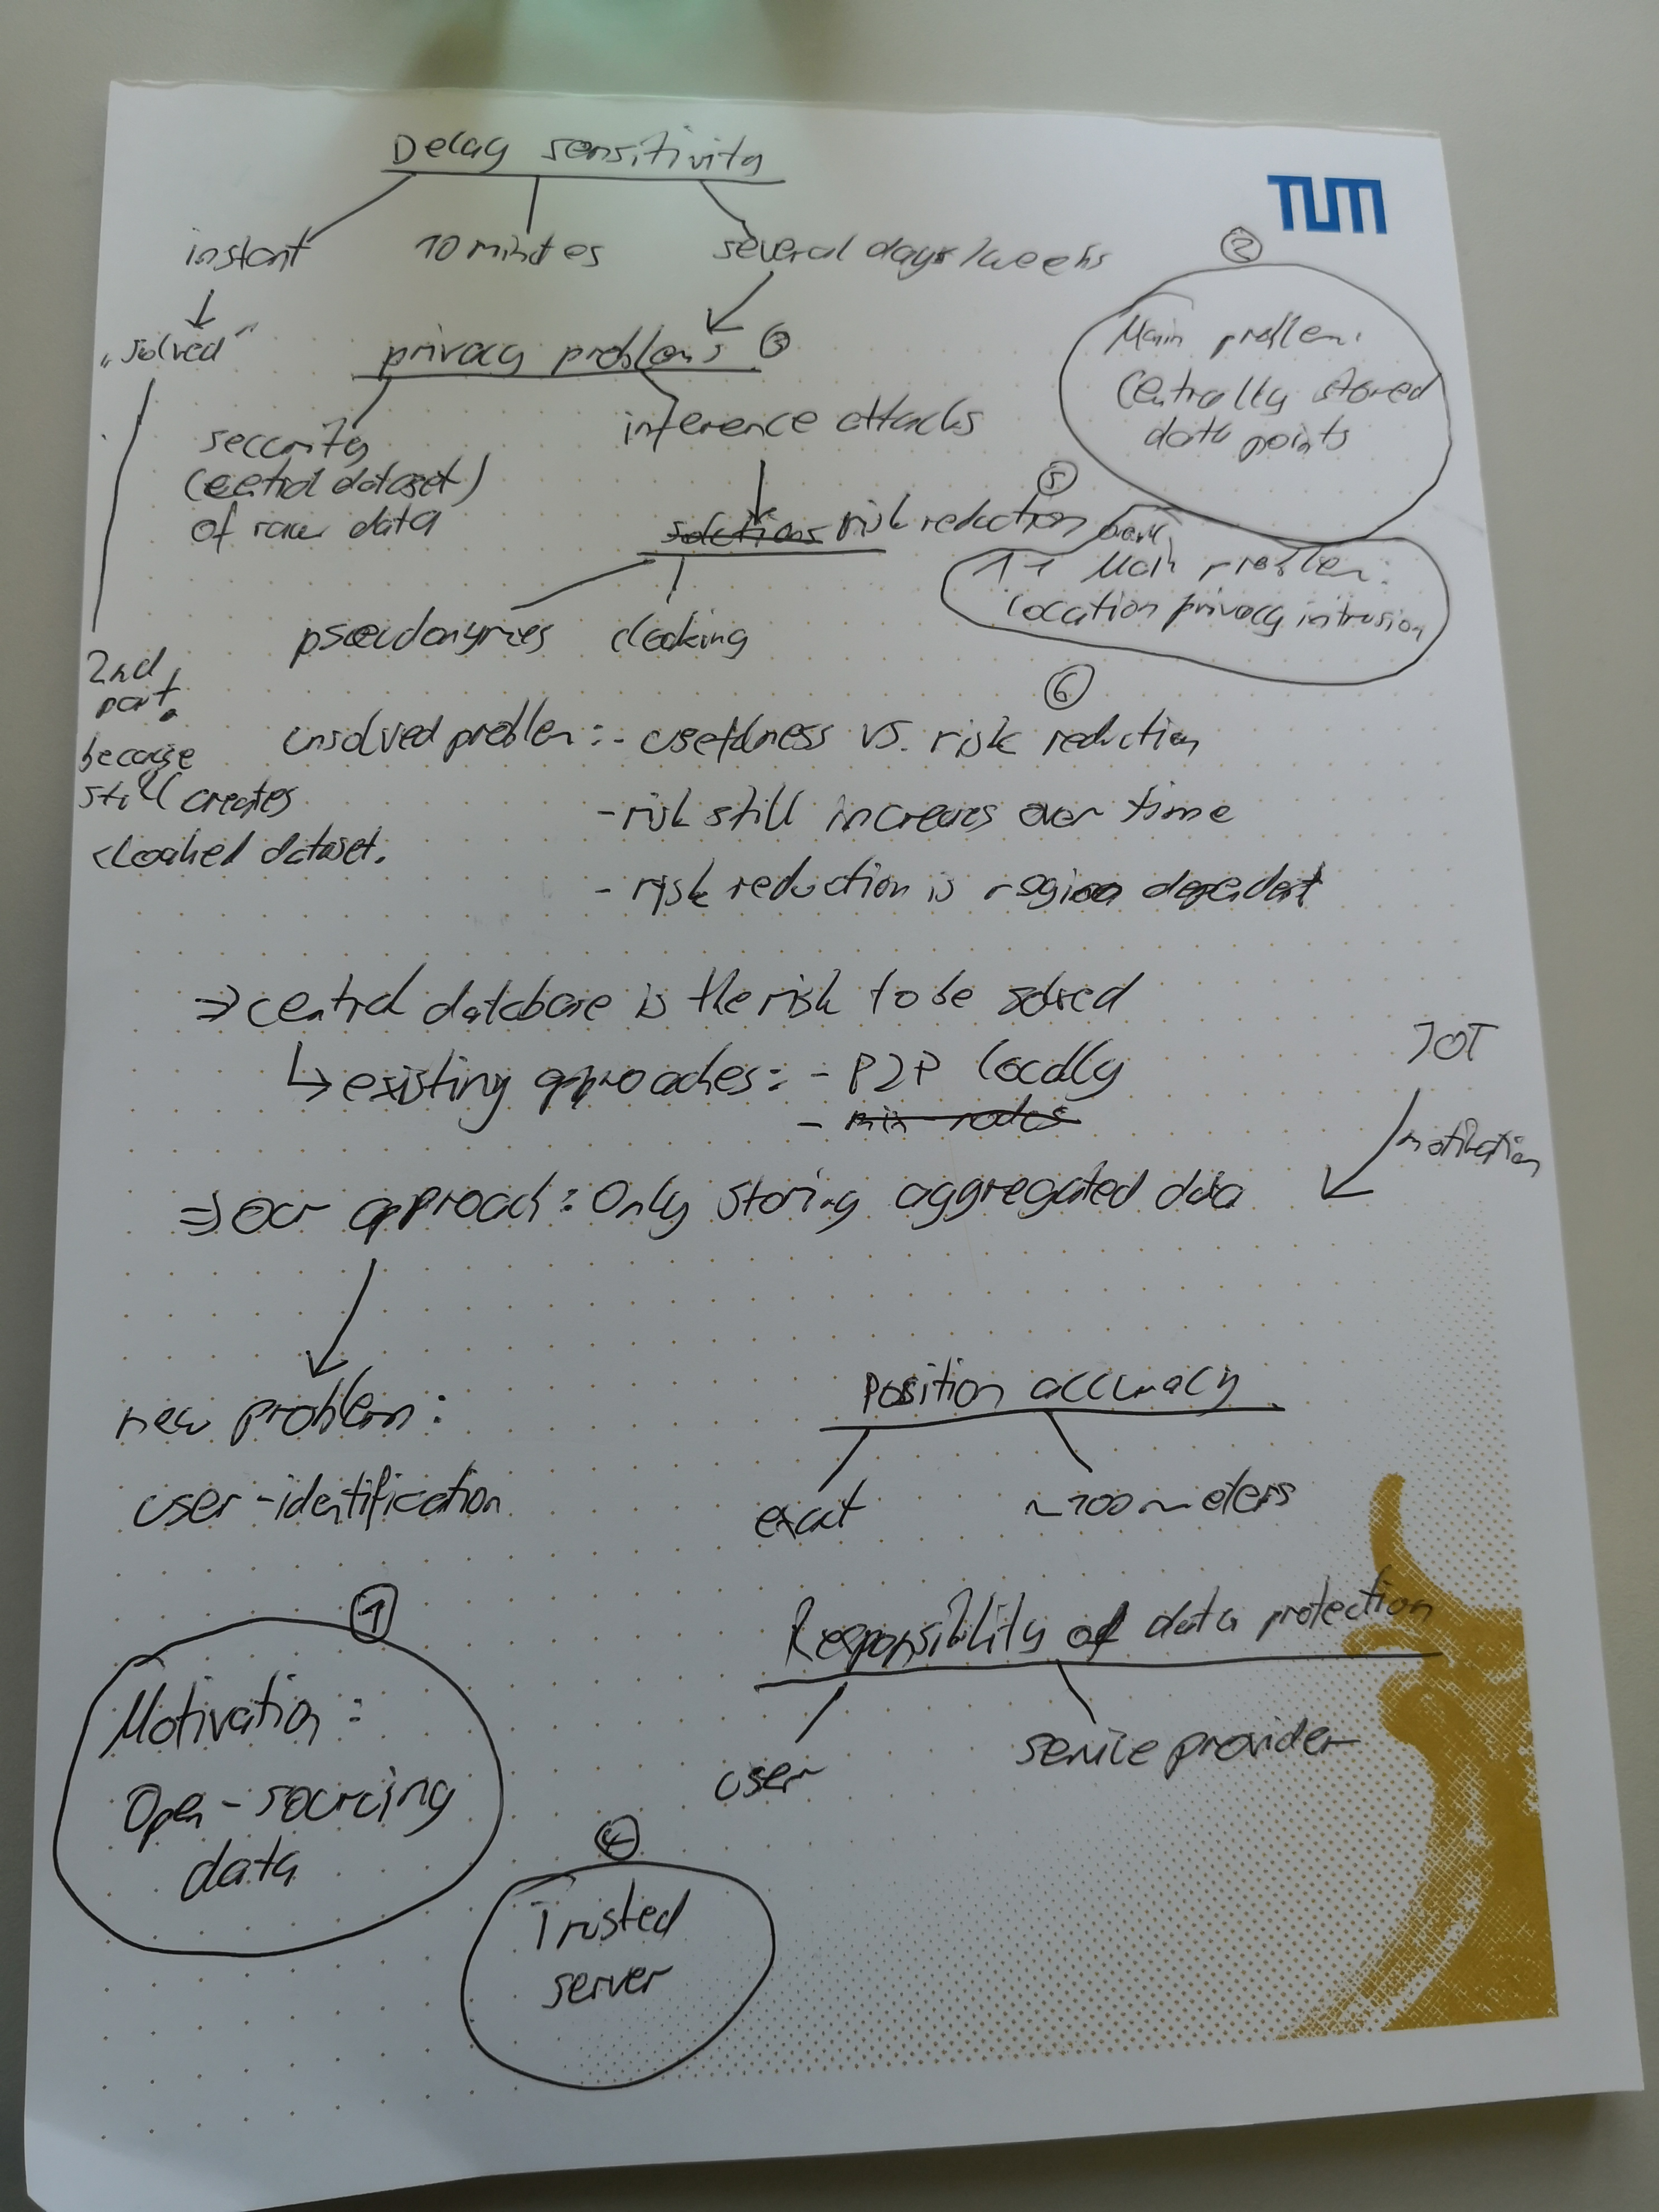
\includegraphics[width=\textwidth]{data/research-overview.jpg}

\section{Summaries of papers}

\parencite{krumm} is one of the first investigating privacy issue in location data. For inferring the home location of a set of car travelling traces of their research subjects, they identify taking the last destination of the car before 3 pm as the most successful among 4 algorithms / heuristics to determine a persons home location. They where able to identify 12.8\% of the users home coordinates. Furthermore by looking up those home coordinates on a free online tool, they are able to retrieve the correct name for about 5\% of the subjects. Nevertheless, those results could be improved by far, as they show that the used data source / white pages are outdated.
In order to protect anonymity, they mainly identify the following different countermeasures:
\begin{itemize}
	\item Pseudonymity: Stripping original IDs from the dataset (by many shown not to be sufficient)
	\item Spatial Cloaking: Application of k-anonymity by hiding all data points in a circle with the center placed randomly around the actual home address
	\item Noise: Adding Gaussian noise to each data point
	\item Rounding: Placing a grid on the location data and mapping each data point to the closest intersection
	\item Dropped Samples: Completely dropping samples in order to reduce the frequency of the data points.
\end{itemize}
Of the application of these countermeasures, only spatial cloaking can preserve data quality, while a Noise with a standard deviation of 5km and a grid for rounding with 5km distances is needed, which render the data useless for many applications.
On the contrary, they showed how easy it is, to make the final step from home location to actual identity. Furthermore, there analyzis is only based on data covering two weeks.


\parencite{cellphone} finds that even when personal data is anonymized thus that names and addresses, etc. are removed, sensitive information can be inferred from the data.
In this study it was shown that from call-records in the US the home address and also often the work address of a person could be inferred.
They highlight that while adhering to the k-anomymity model proposed by \parencite{k-anonymity} it is practically not possible to publish datasets that are still of any significant use.
\\

Also \parencite{privacy-home-work-pairs} highlights the thread that home and work locations can be inferred from anonymized datasets and can in combination with other sources yield even more information about a user. To reduce this risk, they propose "to collect the minimum amount of information needed". In contrary, we want to investigate another approach, so that rich data can still be used and be published in an aggregated manner to let people profit from the data but still preserve privacy.


Another problem that arises is that anonymization algorithms applied to datasets prior to publishing them might yield good results if the location data is in a densily populated area but might perform poorly if the population is only sparse \parencite{time-to-confusion}.

\parencite{time-to-confusion} identify that while privacy algorithms might successfully provide privacy for location data samples in highly frequented areas, but perform poorly and disclose sensitive information for samples in areas with lower traffic frequency. They discuss the problem commonly accepted in research that either the quality of the data becomes poor or useless when applying techniques like k-anonymity \parencite{k-anonymity-old, k-anonymity, k-anonymity-achieving} or that privacy cannot be guaranteed. They propose a novel algorithm based on time-to-confusion. Thus basically whenever it is possible to attribute two different samples of a dataset with a high probability to the same user, the corresponding sample gets removed from the data-set to be published. This is necessary, as "the degree of privacy risk strongly depends on how long an adversary can follow a vehicle" \parencite{time-to-confusion}. In more detail, time-to-confusion also takes into account the entropy information provided by the whole dataset, thus that even when two samples cannot be connected with high probability due to to many possible consecutive samples, analyzing the whole dataset can provide information that actually the possible consecutive samples have different probabilities due to common route choices. E.g. a vehicle on a highway is much more likely to follow on the highway for some more time than leaving the highway. While this information is taken into account, they point out the limitations of their work that when the dataset is matched with street maps, even more samples would have to be remoed to ensure privacy because it will render some former possible consecutive samples impossible due to missing streets connecting them. 

\parencite{location-privacy} introduces the concept of mix-nodes already known from privacy research on a network level (TODO: "copy" related work part of paper "time-to-confusion"). They propose a framework in which privacy is protected through frequently changing pseudonyms. Furthermore they find that similarly to the problem of identifying consecutive samples in \parencite{time-to-confusion}, the change of pseudonyms has also to be obfuscated in order to provide complete privacy. In contrast, this paper focuses mostly on solving the problem that location aware services that e.g. notify you when you are close to a venue of interest, do not need to have access to your location data at anytime but can register to events with a mix-node. Thus they register for the venues of interested and only get notified when the mix-node, which is trusted and has complete access to location data, detects a match. One sees straight away, that this again depends on trust of the users on the mix-node. Nevertheless, the proposed solution of mix-nodes and mix-zones analyzed on a sample shows that even using this framework, privacy cannot be provided, especially as here again the entropy provided by the history of the released or somehow collected data-set makes it too hard to obfuscate the consecutiveness of different pseudonyms.

\parencite{k-anonymity} is the current state of the art of minimum data protection. They define a dataset as the commonly understood tables in SQL. Besides the unique identifier used in the table, a quasi-identifier is the combination of several attributes with which a set of entries can be identified. a dataset adheres to the rules of k-anonymity, if querying every possible such identifier returns at lest a set of k different entries. Thus 1-anonymity identifies an entry exactly and provides no anonymity at all. The anonymity problem arises not from the dataset itself, but from a combination of datasets, that have the attributes of the quasi-identifier in common. This way anonymous knowledge from both datasets can be linked in order to infer information not intended to be made public. They also highlight, that also publishing the same dataset with different privacy-rules, i.e. different anonymization techniques applied, can result in inferences that reveal the original dataset.

\parencite{k-anonymity} clearly highlights that there are two approaches to hiding sensitive information. One is to restrict queries to a database that might reveal sensitive information. In contrast to this approach, they focus on anonymizing the data already before any access to it. Nevertheless, this is based on the assummption that the data owner knows about any possible quasi-identifier in order to obfuscate the dataset sufficiently to provide k-anonymity for all quasi-identifiers. If one quasi-identifier is not thought of, the dataset might expose 1-anonymity for this identifier and result in possible exposures of data not intended to be public.

\parencite{k-anonymity} also discusses further problems that are easy to tackle but nevertheless necessary to protect users' privacy. The order of the published table must be random. Otherwise there is more information (hidden) available that can be used to break k-anonymity. Another problem is when the same table is released and obfuscated differently for the same quasi-identifier, other attributes in the releases can be used to link entries and thus de-anonymize the data.

\parencite{privacy-home-work-pairs} further investigates the fact that from a dataset containing GPS data of trajectories or e.g. twitter-posts as in \parencite{twitter} the home location can be inferred with high probability. They show that also the work location can be identified with pretty high accuracy and probability. Furthermore they find that people who live and work in different regions or more generally, the further work and home diverge, the smaller the anonymity set of the specific user in the dataset and thus the lower also the anonymity. This is similar to the findings of \parencite{location-privacy} that users in less populated areas are exposed to more privacy risk than in denser areas.

\parencite{mix-zones} extends the analyzis of \parencite{location-privacy}.

TODO: Cite approach of disclosure algorithms by \parencite{gruteser2005anonymity}
TODO: Cite confusion approach similar to \parencite{time-to-confusion} by \parencite{hoh2005protecting}
TODO: Read \parencite{tang2006putting}

\subsection{Approaches to avoid central datasets}

\parencite{p2p-android} addresses the possible solution of p2p communication instead of using a central instance. They state, that mobile p2p communication is mainly based on WIFI and bluetooth. They propose a middleware embedded on top of the android operating system to facilitate widespread use of p2p. However, those p2p networks are so far limited to devices close to each other locally, as it works over WIFI or Bluetooth and so far there is no established approach to connect smaller local p2p networks over the internet to completely stop relying on central server instances.

\parencite{crowdsourcing} investigates the problem that in crowdsourcing (with real humans) the reported results, thus the work of the workers allows for inferences about personal information of the (anonymous) worker. To achieve this, they use decentralized computation while "guarantee[ing] security of the proposed protocol". They use as an example the case where a map of publicly available automated external defibrillators is generated through crowdsourcing. Through the reported location data, the privacy of the "worker can be invaded". The state, that so far, only a few have investigated the privacy problems in crowdsourcing (like \parencite{bernstein2011crowdsourcing}). The use a "sum protocol" where sums can be added in an enccrypted way and then be decrypted finally. This is based on the work of \parencite{encryption}. \parencite{lin2005privacy} also find, that this sum protocol is the only way (in crowdsourcing) to guarantee privacy, as otherwise messages between workers would have to be exchanged (our telegram, etc. approach.) In this paper, two other papers are mentioned, that deal with aggregating data while preserving privacy: \parencite{burkhart2010sepia}, \parencite{shamir1979share}. 

\parencite{iot} motivates decentralized data storage and anyalysis as well, though stemming from another motivation. In IoT, bandwith limits require devices to perform decentral analysis and only forward aggregated data to a central database or to aggregate data in a completely decentralized manner. Others, that deal with decentralized analysis are \parencite{bin2010research} and \parencite{tsai2014data}. Furthermore, similar to our motivation, they find that "Especially sectors that deal with highly personalized information, such as healthcare, require according means for the secure and privacy-preserving processing of data". Apparently also \parencite{thrun2004advances} and \parencite{stolpe2011learning} find, that inferring information from data (not location data in this case) is possible. (TODO! read the papers if its correct). Another related source for distributed analysis is \parencite{das2010local}. They define the term "fully decentralized" as where information is only exchanged with local peer nodes. No coordinator is needed thus. Also this paper highlights, that the centralization of data at one single point poses a high risk in case of data theft and furthermore is a single point of failure. They quote from \parencite{carroll2010analysis} that the most power intensive thing in smartphones is receiving and sending data.
For vertically distributed data, as it is also the case for our mobility data, they find five different modi of data analysis:
\begin{itemize}
	\item Central analysis
	\item Local preprocessing, central analysis
	\item Model consensus
	\item Fusion of local models: Each local node builds its own model. Those models are transmitted to a coordinator and fused to a global model
	\item Fusion of local predictions: When a prediction is made, predictions of the single nodes are collected and combined into a consensus
\end{itemize}

\parencite{hoh2006enhancing} also tackle the problem that through to "inference attacks" users can be reidentified even if the location data are anonymized. Especially home locations are easy to infer in suburban scenarios where one person / family belongs to one address. Such sensitive information as home, medical visits, etc. might be inferred. The are also aware that using geo-coded address databases it is easy to infer a person's identity from it's home location. The further quote \parencite{dai2003simulation} (TODO!!) who state that for obtaining "traffic flow information" it is sufficient, if 5\% of all traffic participants send data. To ensure anonymity of data owners, they propose a system in which a trusted third party interacts as mediator between the data owners and the traffic server. The location data is encrypted with the traffic servers public key (private, public key pair) and sent to the third party, using a symmetric encryption algorithm. This way the third party server can confirm the identity of the sender and thus prevent fraud, while it has no access to the data itself, which it forwards to the traffic server. This is a huge advance, but still it is based on a trusted third party server. Also it depends on savely storing (and putting) the symmetric keys into the car / mobile device. They further find that it is necessary to sanitize the incoming data on the traffic server because it might be simply wrong or malicious. This is also necessary in our approach, but in general only, if data is sent as a push variant by devices. In a pull scenario, the data could only be compromised, if somebody manages to attack the application itself. And this can still be handled by sending the aggregation request to different groups in parallel and see whether one request delivers outliers. In addition, they are aware, that the data stored at the traffic server still bears a privacy risk if access to this data is obtained. Thus our approach to totally decentralize the collection and analysis is a huge and necessary step forward. This is especially even more compromising, if one takes road maps into account in order to identify the home locations they find as well. Furthermore, the mapping of a location to an identity is facilitated by white pages like telephone books or real estate records they state. They also report manual inspection in order to map locations to homes which is easy as for most areas there are precise satellite images which help to outrule possibilities. They manage to identify about 27\% of plausible home suggestions from a 239 record data set. (Not validated as exact home location is not revealed in the data set used). Even when data samples are dropped so that there is one GPS point every 10 minutes instead of every minute, still more than 16\% of plausible home locations can be detected. So data suppresion algorithms do reduce the risk of home identification but only to limited extend.

\parencite{casper} tackles the common problem through introduction of a "location anonymiszer" and a "privacy-aware query processor" which enables a user to set its privacy to match k-anonymity (k is variable) and also to choose the degree of spatial-cloaking applied to its data. This approach also requires a trusted third-party (the location anonymizer). Mainly the concept works as following: The third party server receives the exact location data of every user and for each data point creates a new data point through spatial-cloaking that satisfies its privacy setting which then is stored on the server. Whenever a location service (note this approach is mostly for the location-services requiring instant or medium delay data) needs a users location e.g. to notify him about near gas stations (private query), the server receives only the obfuscated location data (a region) and answers with a list of possible matches within this region which is than on the end users device matched with the exact location to retrieve e.g. the nearest gas station. The second benefit is that applications can still reach out to users in a specific area (e.g. to send a promotion to all users in a certain area) through sending this request to the third party which then also replies with a list / area of end users that respects all privacy settings. this is called public query. (On page 764 there might be additional sources - TODO!!). They say that closest to their work is \parencite{gedik2004customizable} (TODO!!!) and \parencite{gruteser2003anonymous} (already read and summarized). Though this still poses the problem of a centralized data set at the query processor. Even the data is pseudonymous and locations are only blurred, other papers like [TODO: cite the others] revealed that even when blurring location data, inference of home locations is still possible. Especially as XXX states, when the data considers rather sparsely trafficed areas. Furthermore identification attacks become more and more precise, the more data points are available (bigger time-span). They further prove, that the overhead of sending a list of possible matches as response to a private query is acceptable (if the data privacy setting is not to strict i.e. k < 50 and cloaked region size < 64 in one region).

\parencite{gruteser2003anonymous} investigates privacy preservation through spatial and temporal cloaking also using a (third party) middleware and a generated location data set. They furthermore talk about the topic that the participant itself should be anonymous (network identifier). This can be achieved in our setting through forwarding a request instead of adding data or sending it to the database in a percentage of cases. They state that this has been investigated by \parencite{chaum1981untraceable} and also many papers refer to onion routing regarding this topic. Also the message size is always padded in order to hinder inferences. They differentiate location services according to three measurements:
\begin{itemize}
	\item Frequency of Access
	\item Time-accuracy / Delay sensitivity
	\item Position accuracy
\end{itemize}
There motivation stems from using sensors already installed in cars instead of separately equipping roads with sensors. This highlights also that our approach is not only limited to location data itself but can be generalized (though usually all information is related to location and time). They state that that for traffic / road information usually high accuracy of the information is not necessary and also a few minutes of delay are tolerable. This highlights, that our approach is also feasible for traffic data and not only pure historical data. They make the example that e.g. harsh breaking data might be used to infer bad road conditions and warn other traffic participants. Regarding this data, huge delays are acceptable as usually a dangerous crossing stays dangerous for a long time (if not forever). They also state that for retrieving nearby points of interest, the time accuracy is high, thus results are needed instantly, but location accuracy does not need to be high. This is in line with the findings of \parencite{casper}. Additionally, they classify threats to privacy into two categories:
\begin{itemize}
	\item Sender anonymity (which can be tackled by us by forwarding with a certain probability)
	\item Inferences of repeated samples (which we tackle by not publishing raw data)
\end{itemize}
The solve this problem by using a (third-party) anonymity server which on the one hand acts as a mix-node and thus solves problem one (also by pseudonyming the data) and also applies cloaking in order to solve the second problem (partially as shown in other papers). They use the definition of anonymity according to k-anonymity (page 35) [Good definition]. They follow an approach that takes time and space into account. If not enough users for k-anonymity where in a certain area, they either apply spatial cloaking (making the data less accurate) or temporal cloaking (gathering in a certain area for a longer time). Also a mixture is possible we think, though then one has to take into account that the same data is not included in different publications. This is also thematized by them using an example and stated that tuples must not overlap in time and space. They find that in their experminental setting, a temporal cloaking of 70 seconds or a spatial one of 250 meters is sufficient (in their setting!) to provide some feeling about the extends. Definition of security as the successfull attempt of an adversary to retrieve data not intended to be public / "violate anonymity constraints". They also talk about the possibility that a user spoofs the service by fake users. We also will address this problem to limit fake users.

\subsection{Infer activities from location data (and publicly available data)}

\parencite{liao2005location} investigates the possibility to label certain times as specific activities (at home, at work, shopping, dining out, visiting, all other) through the use of location data (reduced to the binary variables near restaurant and near store), supervised machine learning and publicly available information of places, etc. They use machine learning and relational markov networkds for it. Also they take transitions into account, e.g. that one does not go from dining out to dining out or also one does usually only dine out a maximum number of times a day. They find that when using data from different subjects, the algorithms can be trained to have an error rate below 20\% when labelling activities, in one experimental setting they even achieve an error rate of 7\%. This shows, that using open source software to infer activities from location data should be pretty accurate right now (the paper is 14 years old right now) so when we infer activities like walking, driving, on a bus, etc. We can assume a pretty low error rate which is in favor of the correctness of our analysis's.

